I% Chapter Template

\chapter{Performance} % Main chapter title

\label{Performance} % Change X to a consecutive number; for referencing this chapter elsewhere, use \ref{ChapterX}

\lhead{Performance. \emph{Performance in practice and Benchmarks}} % Change X to a consecutive number; this is for the header on each page - perhaps a shortened title


%----------------------------------------------------------------------------------------
%	SECTION In practice: Running on JVM
%----------------------------------------------------------------------------------------
\section{In practice: Running on JVM}
\label{InPractice}

In practice, Scala compiles to Java bytecode and executes on a JVM, where we take the Java SE HotSpot as a reference. This imposes additional characteristics of performance that can't be evaluated on the algorithmic level alone.

% code interpreted vs compiled
The JVM use \emph{just in time} (or JIT) compilation of code to take advantage of knowledge about how the code is used at runtime. At first it runs on interpreter mode, it consists of interpreting the bytecode and collecting statistics on the codes execution. Eventually it will compile the code to make it faster using several optimisations and heuristics. The code of the vectors tries to gains performance by aligning with those heuristics and hence taking advantage of the JVM optimizations.

% GC and memory allocations
One of the components of the JVM that will be affected by vectors is the garbage collector. The vector tends to create a large amount of \texttt{Arrays} during transformations, of which many are only necessary for a short time. Those objects will use up memory and possibly degrade performance of future allocations, until the next GC. Having all these unused object will also contribute in an increase in the frequency of GC executions. For that reason the code is optimised to avoid excessive creation of intermediary objects.

% memory access and caches
% system arraycopy primitive
When running on some machine we have several memory cashes helping with performance. The vector tries to align to the underlying cache model to improve performance. The size of the arrays is chosen to take advantage of cache lines while they are copied and traversed. This makes the behaviour of node copies look more as a constant time operation. Further more when copying arrays the \texttt{System.arraycopy} primitive is used. This way, the critical operation that is executed on each update will use the lowest level implementation available for the JVM. This could potentially go down to efficient host machines code when compiled.

%-----------------------------------
%	SUBSECTION Cost of Abstraction
%-----------------------------------
\subsection{Cost of Abstraction and JIT Inline}
% cost of function invokation
One of the optimizations that the JVM provides is function call elimination (abstraction elimination) based on a set of heuristics. This is equivalent to the functions optimisation in section \ref{sec:Abstractions} but done on another level of the pipeline. Critical parts of the code are written with careful detail to match the heuristics of the JVM.

% code compiled (inlined if hot)
% aim to make all critical methods 35< bytes
The optimisation works as follows: the code is run in interpretation mode first while keeping track of statistics on which parts of the code are executed and how many times. When the code is eventually compiled, function calls that are deemed \emph{hot} are inlined. The heuristic favours inline when the function has less than 35 bytes. 

We use this knowledge of the heuristic in two ways. The first is to avoid inlining everything, if the function is small and there is no other optimisation that can be done if inline manual, the code is kept as a function. The second is to inline the methods of the vector API into the clients code. When implementing functions with less than 35 bytes, performance was tested and cross referenced with the VMs inlining diagnostic\footnote{The JVMs \texttt{"-XX:+UnlockDiagnosticVMOptions -XX:+PrintInlining"} flag was used to track the inlining.}. The code was inspected using \texttt{javap -c}, which gives the sizes of the function and helped identifying some optimisation possibilities.

%----------------------------------------------------------------------------------------
%	SECTION Scalameter
%----------------------------------------------------------------------------------------
\section{Measuring performance}
% Scalameter
ScalaMeter framework\cite{scalameter} is used to measure performance of operations on different implementations of vector. This framework was used to spot identify performance improvements or regressions during the development process. 

% warmup to compile code and reduce jitter (JIT, GC)
To have reproducible results with low error margins, ScalaMeter was configured on a per benchmark basis\footnote{The JVM \texttt{-XX:+PrintCompilation} flag vas used to help identifying the ideal configuration.}. Each test is run on 32 different JVM instances to average out badly allocated VMs. On each JVM 32 measurements are taken, while using outlier elimination to remove benchmark runs that where exceptionally different. This could happen if one particular run has a garbage collection, JIT compilation of code or OS executing something else. Before the benchmark runs the JVM is warmed up by running some times the benchmark without taking measurements. During these first execution the VM will be loading classes, taking some statistic on the code and then eventually compiling it.

% types of vectors
There are two main axis of performance comparisons. The first is between the RB-Vector and a perfectly balanced RRB-Tree where the aim is to have an equivalent performance, even if the RRB-Vector have an inherent additional overhead. The second axis is the one that shows the effects of unbalanced nodes on RRB-Tree. For this we compare the same perfect balanced vector with one that is the result of one concatenation of two vectors and with an extremely unbalanced vector. The later vector is generated by concatenating random\footnote{Pseudo random generator where used to be able to reproduce the same ones each time.} small vectors together. The amount of unbalanced nodes is in part affected by the size of the vector. Other axes are discussed in the next section.

%----------------------------------------------------------------------------------------
%	SECTION Generators
%----------------------------------------------------------------------------------------
\section{Implementation Generators}
Until now only one implementation of the RRB-Vector\footnote{Located in the \texttt{scala.collection.immutable.rrbvector} package on GitHub} that is compared against the RB-Vector. But in fact to compare performance on different characteristics like block sizes and concatenation algorithm variant concrete implementations where generated using Scala reflection. Other characteristics involve a complete structure assertion while testing and benchmarks generation. For each combination of characteristics there is a concrete artefact: class implementation, tests and benchmarks.

Code is generated by combining AST using Quasiquotes with some domain specific optimizations. The optimizations are the same that where applied manually on the main implementation of the RRB-Vector. The resulting code is equivalent, except that it lacks formatting. The name of the artefact is used to identify the different characteristics\footnote{All generated artefacts are in the \texttt{scala.collection.immutable.generated.rrbvector} package on GitHub}.

% block sizes
The block sizes used where 32, 64, 128 and 256. 
The main aim is the differences in performances of the operations and identify sizes for which permanence degrades due to loss of cache locality. 
This is the only number in the name of the artefact.

% concat implementation
Both version of the RRB-Vector are to generate vectors. 
This done mostly to compare the performances of other operation on vector that got unbalanced using concatenation. 
\texttt{Complete} (or \texttt{c} in the name of the artefact) is used to name identify the version that rebalances completely the subtree. 
The other one is named \texttt{Quick} or \texttt{q} in the name of the artefact.

% testing
For testing purposes, for each implementation there is a second one generated with heavy assertions on the whole structure of the vector on most methods (see \ref{InvariantAssertions}). 
Concrete benchmarks are also generated at the same time.

Generating this code was the only reasonable way to implement this huge amount of classes while implementing new features on them. 
Changes that would otherwise had to be propagated by hand on each one. 
This also help to find and fix bugs, because a bug has a higher probability of affecting at leas one of the artefact and a fixed bug fixes it on all of them.

%----------------------------------------------------------------------------------------
%	SECTION Benchmarks
%----------------------------------------------------------------------------------------
\section{Benchmarks}
% reiterate the the different benchmark types 
%% differences between implementation (vector vs rrbvector)
%% differences between unbalances
%% differences between block sizes
%% differences between concatenation rebalancing method
% benchmarks on core operations
\color{red} TODO \color{black}

%-----------------------------------
%	SUBSECTION Apply
%-----------------------------------
\subsection{Apply}
% describe the benchmark function
% compare expectation with results
% explain the upper bound
% explain apparently incoherent results
\color{red} TODO \color{black}

\begin{figure}[h!]
  \centering
  \includegraphics[width=\textwidth]{Benchmarks/Apply_2.pdf}
  \includegraphics[width=\textwidth]{Benchmarks/Apply_3.pdf}
  \label{ApplyBenchmarks}
  \caption{Time to execute 10k apply operations on sequential indices.}
\end{figure}

\begin{figure}[h!]
  \centering
  \includegraphics[width=\textwidth]{Benchmarks/Apply_random_3.pdf}
  \label{ApplyRandomBenchmarks}
  \caption{Time to execute 10k apply operations on random indices.}
\end{figure}

\begin{figure}[h!]
  \centering
  \includegraphics[width=0.49\textwidth]{Benchmarks/Apply_blocks_32.pdf}
  \includegraphics[width=0.49\textwidth]{Benchmarks/Apply_blocks_64.pdf}
  \includegraphics[width=0.49\textwidth]{Benchmarks/Apply_blocks_128.pdf}
  \includegraphics[width=0.49\textwidth]{Benchmarks/Apply_blocks_256.pdf}
  \label{ApplyBlocksBenchmarks}
  \caption{Time to execute 10k apply operations on sequential indices. Comparing performances for different block sizes and different implementation of the concatenation inner branch rebalancing (Complete/Quick).}
\end{figure}

%-----------------------------------
%	SUBSECTION Concatenation
%-----------------------------------
\subsection{Concatenation}
% describe the benchmark function
% compare expectation with results
% explain the upper bound
% explain apparently incoherent results
\color{red} TODO \color{black}

\begin{figure}[h!]
  \centering
  \includegraphics[width=\textwidth]{Benchmarks/Concat.png}
  \label{ConcatBenchmarks}
  \caption{Execution time for a concatenation operation on two vectors. In theory (and in practice) Vector concatenation is $O(left + right)$ and the rrbVector concatenation operation is $O(log_{32}(left + right))$.}
\end{figure}

%-----------------------------------
%	SUBSECTION Append
%-----------------------------------
\subsection{Append}
% describe the benchmark function
% compare expectation with results
% explain the upper bound
% explain apparently incoherent results

\color{red} TODO \color{black}

\begin{figure}[h!]
  \centering
  \includegraphics[width=\textwidth]{Benchmarks/Append_2.pdf}
  \label{Append2Benchmarks}
  \caption{Time to execute 256 append operations. This shows the amortized cost of the append operation.}
\end{figure}

\begin{figure}[h!]
  \centering
  \includegraphics[width=\textwidth]{Benchmarks/Append_3.pdf}
  \label{Append3Benchmarks}
  \caption{Time to execute 256 append operations. This shows the amortized cost of the append operation.}
\end{figure}

\begin{figure}[h!]
  \centering
  \includegraphics[width=0.49\textwidth]{Benchmarks/Append_blocks_32.pdf}
  \includegraphics[width=0.49\textwidth]{Benchmarks/Append_blocks_64.pdf}
  \includegraphics[width=0.49\textwidth]{Benchmarks/Append_blocks_128.pdf}
  \includegraphics[width=0.49\textwidth]{Benchmarks/Append_blocks_256.pdf}
  \label{IterationBlocksBenchmarks}
  \caption{Time to execute 256 append operations. This shows the amortized cost of the append operation. Comparing performances for different block sizes and different implementation of the concatenation inner branch rebalancing (Complete/Quick).}
\end{figure}

%-----------------------------------
%	SUBSECTION Prepend
%-----------------------------------
\subsection{Prepend}
% describe the benchmark function
% compare expectation with results
% explain the upper bound
% explain apparently incoherent results
\color{red} TODO \color{black}

\begin{figure}[h!]
  \centering
  \includegraphics[width=\textwidth]{Benchmarks/Prepend_2.pdf}
  \includegraphics[width=\textwidth]{Benchmarks/Prepend_3.pdf}
  \label{PrependBenchmarks}
  \caption{Time to execute 256 prepend operations. This shows the amortized cost of the prepend operation.}
\end{figure}

\begin{figure}[h!]
  \centering
  \includegraphics[width=0.49\textwidth]{Benchmarks/Prepend_blocks_32.pdf}
  \includegraphics[width=0.49\textwidth]{Benchmarks/Prepend_blocks_64.pdf}
  \includegraphics[width=0.49\textwidth]{Benchmarks/Prepend_blocks_128.pdf}
  \includegraphics[width=0.49\textwidth]{Benchmarks/Prepend_blocks_256.pdf}
  \label{PrependBenchmarks}
  \caption{Time to execute 256 prepend operations. This shows the amortized cost of the append operation. Comparing performances for different block sizes and different implementation of the concatenation inner branch rebalancing (Complete/Quick).}
\end{figure}


%-----------------------------------
%	SUBSECTION Splits
%-----------------------------------
\subsection{Splits}
% describe the benchmark function
% compare expectation with results
% explain the upper bound
% explain apparently incoherent results
\color{red} TODO \color{black}

\begin{figure}[h!]
  \centering
  \includegraphics[width=\textwidth]{Benchmarks/Split_take_3.pdf}
  \includegraphics[width=\textwidth]{Benchmarks/Split_drop_3.pdf}
  \label{SplitsBenchmarks}
  \caption{Execution time of take and drop.}
\end{figure}


%-----------------------------------
%	SUBSECTION Iterator
%-----------------------------------
\subsection{Iterator}
% describe the benchmark function
% compare expectation with results
% explain the upper bound
% explain apparently incoherent results: iteration of sightly unbalanced vector is faster
\color{red} TODO \color{black}

\begin{figure}[h!]
  \centering
  \includegraphics[width=\textwidth]{Benchmarks/Iteration_3.pdf}
  \includegraphics[width=\textwidth]{Benchmarks/Iteration_4.pdf}
  \label{IterationBenchmarks}
  \caption{Excecution time to iterate through all the elements of the vector.}
\end{figure}

\begin{figure}[h!]
  \centering
  \label{IterationBlocksBenchmarks}
  \includegraphics[width=0.49\textwidth]{Benchmarks/Iteration_blocks_32.pdf}
  \includegraphics[width=0.49\textwidth]{Benchmarks/Iteration_blocks_64.pdf}
  \includegraphics[width=0.49\textwidth]{Benchmarks/Iteration_blocks_128.pdf}
  \includegraphics[width=0.49\textwidth]{Benchmarks/Iteration_blocks_256.pdf}
  \caption{Excecution time to iterate through all the elements of the vector. Comparing performances for different block sizes and different implementation of the concatenation inner branch rebalancing (Complete/Quick).}
\end{figure}

%-----------------------------------
%	SUBSECTION Builder
%-----------------------------------
\subsection{Builder}
% describe the benchmark function
% compare expectation with results
% explain the upper bound
% explain apparently incoherent results
\color{red} TODO \color{black}

\begin{figure}[h!]
  \centering
  \includegraphics[width=\textwidth]{Benchmarks/Builder_3.pdf}
  \includegraphics[width=\textwidth]{Benchmarks/Builder_4.pdf}
  \label{BuilderBenchmarks}
  \caption{Execution time to build a vector of a given size.}
\end{figure}

\begin{figure}[h!]
  \centering
  \includegraphics[width=\textwidth]{Benchmarks/Builder_blocks.pdf}
  \label{BuilderBlocksBenchmarks}
  \caption{Execution time to build a vector of a given size. Comparing performances for different block sizes.}
\end{figure}

%-----------------------------------
%	SUBSECTION Parallel split-combine
%-----------------------------------
\subsection{Parallel split-combine}
% describe the benchmark function
% compare expectation with results
% explain the upper bound
% explain apparently incoherent results
\color{red} TODO \color{black}

\begin{figure}[h!]
  \centering
  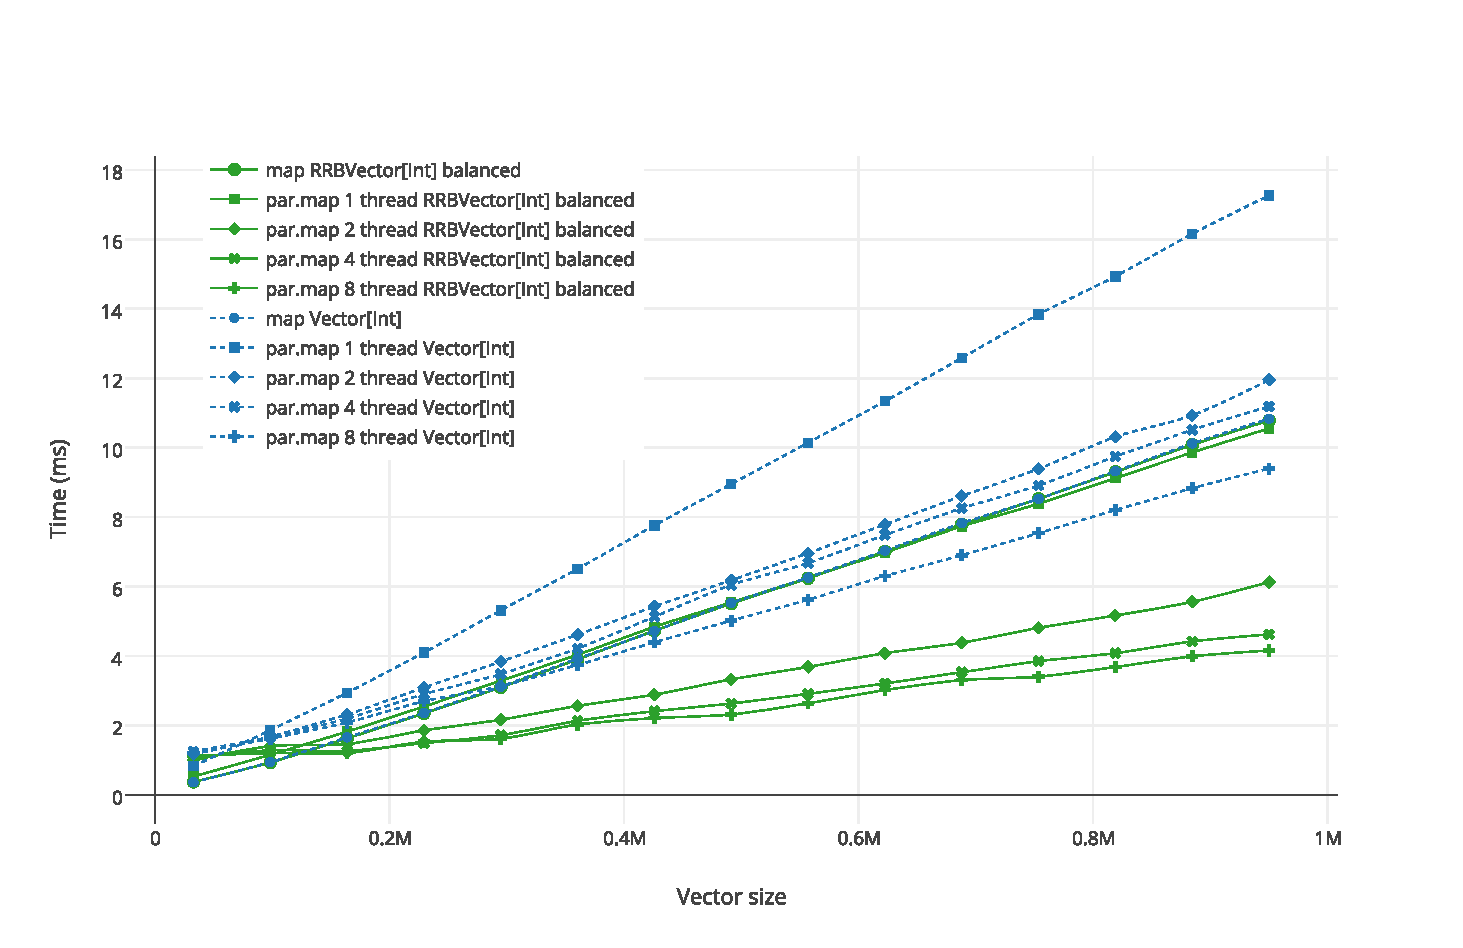
\includegraphics[width=\textwidth]{Benchmarks/Parmap_balanced.pdf}
  \label{ParallelBenchmarks}
  \caption{Benchmark on map and parallel map using the function (\textsc{x=>x}) to show the difference time used in the framework. This time represents the time spent in the splitters and combiners of the parallel collection (iterator and builder for the sequential version).}
\end{figure}

\begin{figure}[h!]
  \centering
  \includegraphics[width=0.49\textwidth]{Benchmarks/parmap_unbalanced_1.pdf}
  \includegraphics[width=0.49\textwidth]{Benchmarks/parmap_unbalanced_2.pdf}
  \includegraphics[width=0.49\textwidth]{Benchmarks/parmap_unbalanced_4.pdf}
  \includegraphics[width=0.49\textwidth]{Benchmarks/parmap_unbalanced_8.pdf}
  \label{ParallelUnbalancedBenchmarks}
  \caption{Benchmark on map and parallel map using the function (\textsc{x=>x}) to show the difference time used in the framework. This time represents the time spent in the splitters and combiners of the parallel collection.}
\end{figure}


%-----------------------------------
%	SUBSECTION Memory footprint
%-----------------------------------

\subsection{Memory footprint}
% describe the benchmark function
% compare expectation with results
% explain the upper bound
% explain apparently incoherent results
\color{red} TODO \color{black}

\begin{figure}[h!]
  \centering
  \includegraphics[width=\textwidth]{Benchmarks/Memory_3.pdf}
  \includegraphics[width=\textwidth]{Benchmarks/Memory_blocks.pdf}
  \label{MemoryFootprints}
  \caption{Memory Footprint}
\end{figure}



